\documentclass{beamer}
\usepackage[latin1]{inputenc}
\usepackage[T1]{fontenc}
\usepackage{fixltx2e}
\usepackage{graphicx}
\usepackage{longtable}
\usepackage{float}
\usepackage{wrapfig}
\usepackage{soul}
\usepackage{textcomp}
\usepackage{marvosym}
\usepackage{wasysym}
\usepackage{latexsym}
\usepackage{amssymb}
\usepackage{hyperref}
\usepackage{url}
\usepackage{verbatim}
\tolerance=1000
\usepackage[english]{babel} \usepackage{ae,aecompl}
\usepackage{mathpazo,courier,euler} \usepackage[scaled=.95]{helvet}
\usepackage{listings}
\lstset{
  language=TeX,
  basicstyle=\ttfamily\bfseries,
  commentstyle=\ttfamily\color{blue},
  stringstyle=\ttfamily\color{orange},
  showstringspaces=false,
  breaklines=true,
  postbreak = \space\dots
}

\newcommand{\typ}[1]{\lstinline{#1}}

\mode<presentation>
{
  \usetheme{Warsaw}
  \useoutertheme{infolines}
  \setbeamercovered{transparent}
}


\title{FOSSEE}
\institute[IIT Bombay] {IIT Bombay}
\date{}

\begin{document}

% Document title
\begin{frame}
   \begin{center}
   \maketitle  
   
\includegraphics[scale=2]{fossee.png} \\
   \end{center}
\end{frame}


\section{Introduction}
\begin{frame}
  \frametitle{{FOSSEE} - Introduction}
  \begin{itemize}
  \item Free and Open source Software for Science and Engineering Education 
  \item Based at IIT Bombay
  \item Goal: Promote the use of open source software tools among students and facutly of Science and Engineering colleges/institutes/universities across India.
  \item Funded by MHRD as part of National Mission on Education through ICT
  \end{itemize}  
\end{frame}

\section{Principal Investigators}
\begin{frame}
  \frametitle{Principal Investigators of the Project}
  \begin{itemize}
  \item Prof. Prabhu Ramachandran
  \item Prof. Madhu Belur
  \item Prof. Kannan Moudgalya
  \item Prof. Mani Bhushan
  \end{itemize}
\end{frame}


\section{What do we do?}
\begin{frame}
  \frametitle{Projects of FOSSEE}
  \begin{center}
  	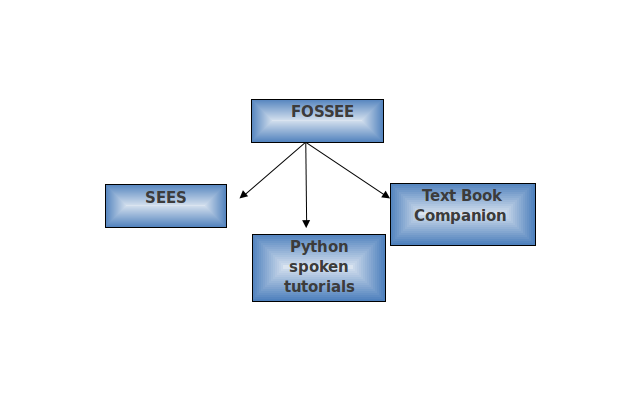
\includegraphics[scale=0.25]{st.png}
  \end{center}
\end{frame}

\section{SEES}
\begin{frame}
  \frametitle{SEES}
    \begin{itemize}
    \item Objective: Help students to use open source software tools for curricular purposes. 
    \item Software Engineering for Engineers and Scientists.
    \item For students of BE/BTech and ME/MTech programmes(Non CS/IT Streams)
    \item Modules 
    \begin{itemize}
    \item Using Linux Tools
	\item Basic Python Programming
	\item LateX
	\item Version Control
	\item Test Driven Development
	\item Advanced Python
    \end{itemize}
	\end{itemize}
\end{frame}

\section{Workshop}

\begin{frame}
  \frametitle{Workshop}
  \begin{itemize}
  \item Objective: Advantages of using Free and Open Source Software (FOSS)
  \item For: Coordinators on "Software Development Techniques for Teachers of Engineering and Science Institutes"
  \item Conducted in 2 parts.
  \begin{enumerate}
  \item Expert faculty from remote centers to a Coordinators training workshop in IIT.
  \item At selected remote centers, lecture and live transmission takes place through distance mode using AVIEW technology. 
  \end{enumerate}
  \item \url{{http://goo.gl/6puaI}}
  \end{itemize}
\end{frame}


\section{Textbook Conversion}

\begin{frame}	
	\frametitle{Textbook Conversion}
	\begin{itemize}
	\item Objective: Create a repository of reference material in the form of solved problems for Scientific Computing with Open Source tools.
	\item How does it work?
	\item How do I contribute?
	\item For more details visit {\url{http://fossee.in/textbooks/}}
	\end{itemize}
\end{frame}

\section{Spoken Tutorials}

\begin{frame}
	\frametitle{Spoken Tutorials}
	\begin{itemize}
	\item Objective: Create video tutorials on various modules of Python
	\item Completed: 37 video tutorials related to scientific computing using python.
	\item Ongoing: Video tutorials on the remaining modueles in SEES course
	\item Can be used for self learning and teaching purposes
	\item Videos can be downloaded from http://fossee.in/stvideos	
	\end{itemize}
\end{frame}


\begin{frame}
\frametitle{}   
  \begin{center}
    \Huge{Thank You!}
  \end{center}
\end{frame}


\end{document} 
 
